\documentclass[xcolor=table]{beamer}

\usetheme[secheader,compress]{Madrid} %Primary theme

\usepackage{verbatim}
\usepackage{graphicx}
\usepackage{hyperref}

%% UTM Colors
\definecolor{UTMblue}{rgb}{0.043137, 0.137254, 0.254901}
\definecolor{UTMorange}{rgb}{1.0, 0.509803, 0}

\setbeamercolor{palette primary}{bg=UTMblue,fg=white}
\setbeamercolor{palette secondary}{bg=UTMblue,fg=white}
\setbeamercolor{palette tertiary}{bg=UTMblue,fg=white}
\setbeamercolor{palette quaternary}{bg=UTMblue,fg=white}
\setbeamercolor{structure}{fg=UTMblue} % itemize, enumerate, etc
\setbeamercolor{section in toc}{fg=UTMblue} % TOC sections
\setbeamercolor{title}{fg=UTMorange}

\setbeamercolor{subsection in head/foot}{bg=UTMorange,fg=white}

%%%%%%%%%%% BEGIN MACROS %%%%%%%%%%%%%%%%%%
% frameT: Frame with title
\newcommand{\frameT}[2]{\frame{\frametitle{#1} #2}}

% frameF: Fragile frame with title
\newcommand{\frameF}[2]{
  \begin{frame}[fragile]
    \frametitle{#1}
    #2
  \end{frame}
}

% frameTop: Frame aligned t the top
\newcommand{\frameTop}[2]{\frame[t]{\frametitle{#1} #2}}


\newcommand{\tab}{\hspace{1cm}}

\newcommand{\spaceor}{\hspace{5pt} \textbf{or} \hspace{5pt}}

%%%%%%%%%%% END MACROS %%%%%%%%%%%%%%%%%%%%



\begin{document}

\title{Gardener's Best Friend}

\author{Shakira Perry, Lucy Gauldin, Vrushank Mali, and Wesley Duclos}
\institute{UT-Martin}
\date{\today}

%%%%%%%%%%% BEGIN TITLE %%%%%%%%%%%%%%%%%%
\frame{\titlepage}

 %\section{Outline}
%%%%%%%%%%%% END TITLE  %%%%%%%%%%%%%%%%%%


\section{Introduction}
\frameT{Motivation} {
  So why did we pick this project?
\begin{columns}
\column{0.5\textwidth}
   \begin{enumerate}
    \item Love of plants
      \bigskip
    \item Keep plants ALIVE!!!
    \bigskip
    \item Improve plant health
  \end{enumerate}
\column{0.5\textwidth}
    \begin{figure}[H]
    
\includegraphics[width = .7\linewidth]{app_logo.png}
    \end{figure}
    \end{columns}

  
}



\frameT{Project Goals} {
  So what do we think we need to have?
\bigskip

\begin{itemize}
    \item \textbf{Plant Journal}
          \begin{itemize} 
            \item Keep record of plant's health with journal entries.
          \end{itemize}
    \item \textbf{Photo records}
        \begin{itemize}
            \item Journal entries will contain photos that can be updated by the user.
        \end{itemize}

    \item \textbf{Calendar Reminders}
        \begin{itemize}
            \item Depending on the schedule assigned by the user, a reminder will be sent to water their plants.
        \end{itemize}

        \item \textbf{Plant Information}
        \begin{itemize}
            \item If the plant is within the app's database, the user will be presented further information about their plant's care.
        \end{itemize}
        
    
\end{itemize}
}

\begin{frame}[fragile]
\frametitle{Technology}
\begin{columns}
\column{0.5\textwidth}
Technology used:
\bigskip
   \begin{enumerate}
    \item Android Studio
    \bigskip
    \item Kotlin programming language
    \bigskip
    \item SQLite
    \bigskip
    \item Plant API from Perenual
    \bigskip
    \item GitHub
  \end{enumerate}
\column{0.5\textwidth}
    \begin{figure}[H]
    
\includegraphics[width = .8\linewidth]{technologies.png}
    \end{figure}
    \end{columns}
\end{frame}

\begin{frame}[fragile]
\frametitle{Android Studio}
\begin{columns}
\column{0.5\textwidth}
   \begin{enumerate}
    \item Integrated Development Environment
    \bigskip
    \item Developed By Google
    \bigskip
    \item Based on IntelliJ IDEA
    \bigskip
    \item Emulator
    \bigskip
    \item LINT Checker
    \bigskip
    \item Android Jetpack
  \end{enumerate}
\column{0.5\textwidth}
    \begin{figure}[H]
    \includegraphics[width = .8\linewidth]{AndroidStudio.png}
    \end{figure}
    \end{columns}
\end{frame}

\begin{frame}[fragile]
\frametitle{Kotlin}
\begin{columns}
\column{0.5\textwidth}
   \begin{enumerate}
    \item Official Language for Android
    \bigskip
    \item Interoperability
    \bigskip
    \item Comprehensive Standard Library
    \bigskip
    \item Multiplatform Development
    \bigskip
    \item Gradle Support
    \bigskip
    \item Concise and Readable
    
  \end{enumerate}
\column{0.5\textwidth}
    \begin{figure}[H]
    \includegraphics[width = .8\linewidth]{Kotlin.png}
    \end{figure}
    \end{columns}
\end{frame}

\begin{frame}[fragile]
\frametitle{SQLite}
\begin{columns}
\column{0.5\textwidth}
   \begin{enumerate}
    \item Embedded Database
    \bigskip
    \item Zero Configuration
    \bigskip
    \item ACID Compliant
    \bigskip
    \item Cross-platform
    \bigskip
    \item Highly Reliable
    \bigskip
    \item Low Maintainance
  \end{enumerate}
\column{0.5\textwidth}
    \begin{figure}[H]
    \includegraphics[width = .8\linewidth]{SQLite.jpeg}
    \end{figure}
    \end{columns}
\end{frame}

\begin{frame}[fragile]
\frametitle{Plant API from Perenual}
\begin{columns}
\column{0.5\textwidth}
   \begin{enumerate}
    \item Plant Marketplace
    \bigskip
    \item Based on RESTful API
    \bigskip
    \item Stateless
    \bigskip
    \item Uniform Interface
    \bigskip
    \item Cacheability
    \bigskip
    \item Security
  \end{enumerate}
\column{0.5\textwidth}
    \begin{figure}[H]
    \includegraphics[width = .8\linewidth]{Perenual.png}
    \end{figure}
    \end{columns}
\end{frame}

\begin{frame}[fragile]
\frametitle{Github}
\begin{columns}
\column{0.5\textwidth}
   \begin{enumerate}
    \item Version Control
    \bigskip
    \item Code Hosting
    \bigskip
    \item Collaboration
    \bigskip
    \item Branches
    \bigskip
    \item Security Features
   \bigskip 
    \item Code Search
  \end{enumerate}
\column{0.5\textwidth}
    \begin{figure}[H]
    \includegraphics[width = .8\linewidth]{Github.png}
    \end{figure}
    \end{columns}
\end{frame}

\frameT{Journey to the App}
{
First Mockup \\

\begin{center}
   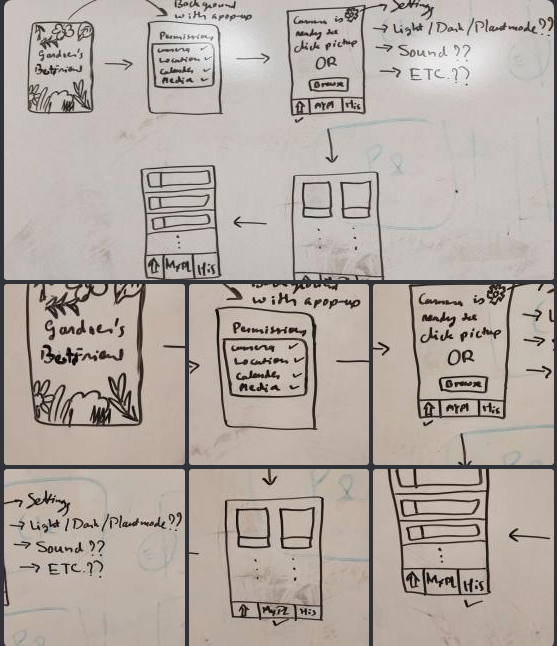
\includegraphics[scale=0.35]{Screenshot 2023-09-30 183429.png}
\end{center}
}

\frameT{Page Mockups}
{
\centering
\begin{subfigure}
  \centering
  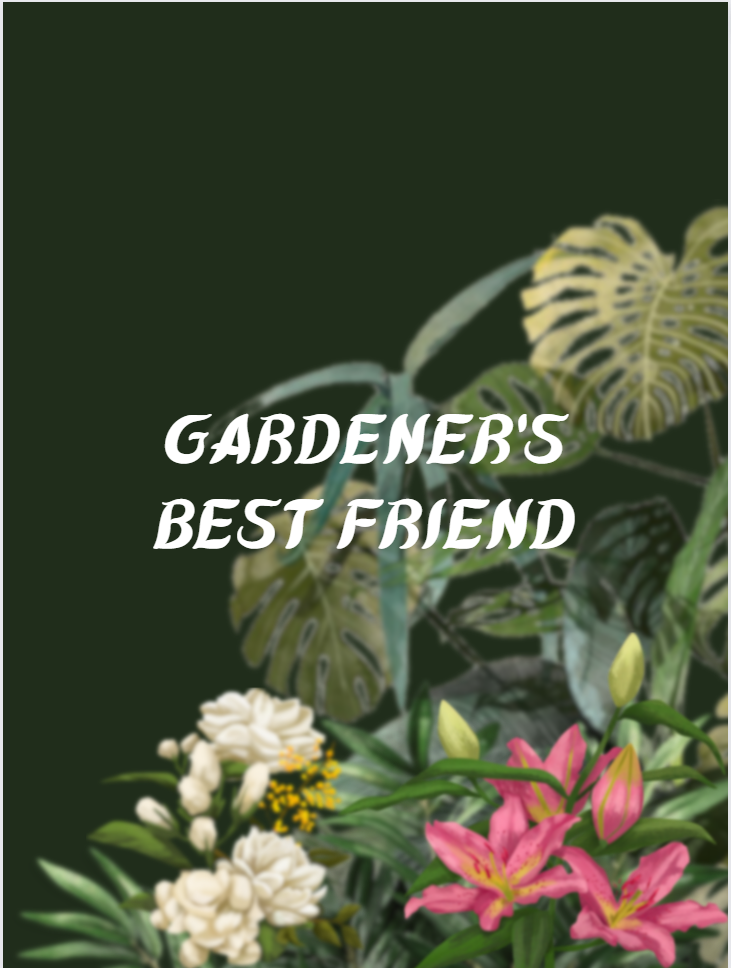
\includegraphics[scale = .3]{Screenshot 2023-09-30 183202.png}
\end{subfigure}%
\begin{subfigure}
  \centering
  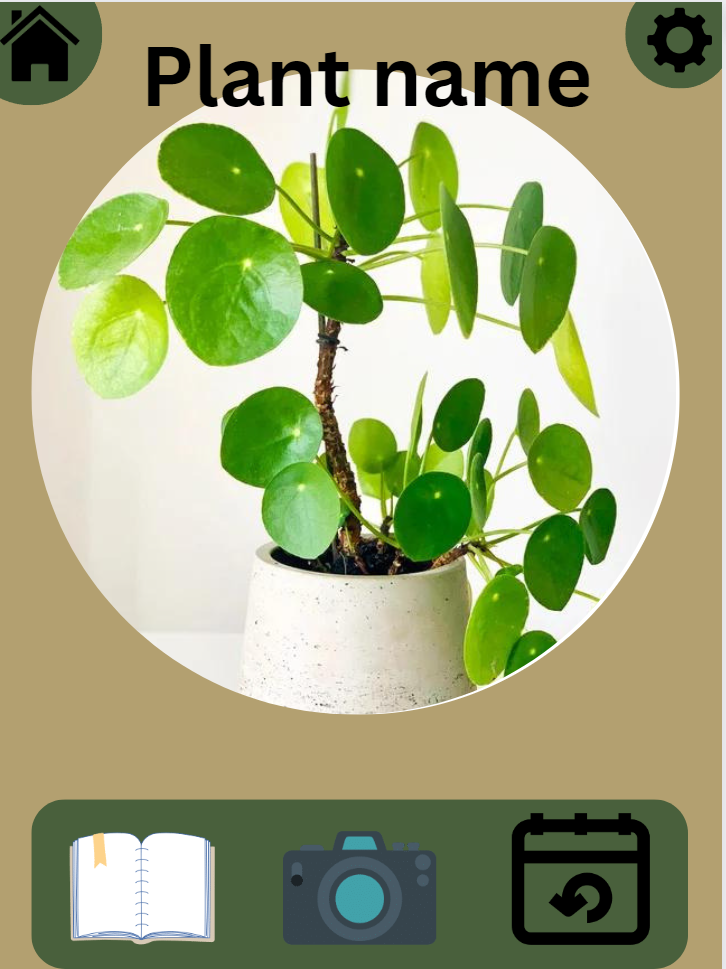
\includegraphics[scale = .3]{Screenshot 2023-09-30 183239.png}
\end{subfigure}
\label{fig:test}
}

\frameT{Page Mockups 2}
{
\centering
\begin{subfigure}
  \centering
  \includegraphics[scale = 1]{Screenshot 2023-11-06 205537.png}
\end{subfigure}%
\begin{subfigure}
  \centering
  \includegraphics[scale = 1]{Screenshot 2023-11-06 205547.png}
\end{subfigure}
\label{fig:test}
}

\frameT{Page Mockups 3}
{
\centering
\begin{subfigure}
  \centering
  \includegraphics[scale = 1]{Screenshot 2023-11-06 205551.png}
\end{subfigure}%
\begin{subfigure}
  \centering
  \includegraphics[scale = 1]{Screenshot 2023-11-06 205600.png}
\end{subfigure}
\label{fig:test}
}

\frameT{Demonstration} {
\begin{center}
  \href{https://youtu.be/QgudUSF5qa4}{Demonstration Video}  
\end{center}

}





\frameT{Results} {

  \bigskip

  Things that worked?

  \bigskip

  Things that didn't work?\\
  Mixing Java Database and SQLite

  \bigskip
  Challenges? \\
  Permissions\\
  Reminders\\
  Database Storage and Retrieval \\
Android Studio communicating with Github for version control \\
  Deciding on what features the app needed
}

\frameT{Conclusions} {
  While it has been a fun yet challenging project, there is a lot more left to do.
  \begin{itemize}
      \item Journal entry storage for retrieval.
      \bigskip
      \item Access  API database.
  \end{itemize}
}

\frameT{Any Questions?} {
  
  \begin{center}
    Questions?
  \end{center}
  \begin{center}
    Comments?
  \end{center}

  \bigskip
\begin{center}
GitHub Repo: https://github.com/shaaperr/GardenersBestFriend \\
\bigskip
  Further project/author information: \\
 Wesley Duclos: wescducl@ut.utm.edu \\ Lucy Gauldin: bildgaul@ut.utm.edu \\ Vrushank Mali: vrujmali@ut.utm.edu \\ 
       Shakira Perry: shaaperr@ut.utm.edu

  
    \includegraphics[width=4cm]{happyplant.png}
  \end{center}
}

%\frameF{fragile test} {
%}

%% \frameF{Prolog Family Tree} {
%% \begin{verbatim}
%% hello
%% \end{verbatim}



%% }

%Empty Page
%\frameT{Frame 1}{
%}  


\end{document}